\section{Using Cisco}\label{sec:cisco_usage}
The Cisco localisation and positioning system is already in use at Aalborg University. To be able to use the information from the system, we had a meeting with the MSE administrator, during which he raised concerns for privacy, because of the legality of storing person sensitive data, as mentioned in \cref{sec:permission}. 

Furthermore the MSE administrator wishes to be able to provide the location data to future student projects with ease. To accommodate this, it has been asked of us to build and deploy an intermediate service with the goal of obfuscating sensitive personal data, such as MAC addresses and user names. This service is intended to duplicate the functionality of the Cisco MSE RESTful API, such that it acts as a transparent proxy. This is achieved by creating an intermediate RESTful service, that simply redirects requests and processes the response before sending it back to the initial requester, as illustrated on \cref{fig:cisco_usage}.

\begin{figure}[ht]
	\begin{center}
	\includegraphics[scale=0.9]{graphics/cisco_usage.png}
	\caption{Cisco usage}
	\label{fig:cisco_usage}
	\end{center} 
\end{figure}

There are several different methods to obfuscate personal sensitive data such as MAC addresses. To accommodate the ability to analyse and predict crowd movement, we do not need to be able to uniquely identify devices. As a consequence we choose one of the least computation-heavy methods; overwriting the MAC addresses with the word \emph{OBFUSCATED}. The obfuscation is not performed if a user has agreed to let us save their MAC address.
This is a simple solution that makes sure the server does not store any sensitive data without the acceptance of the user. The solution accommodates current needs, and we expect more requirements will be added as the application groups start using the location data.

A RESTful service typically communicates using the HTTP or HTTPS protocols, and functions by receiving requests for specific data resources, called Uniform Resource Identifiers (URIs) to which it responds by sending the requested data. As an example we can send a HTTPS GET request to 64.103.26.61, which is a Cisco MSE test server, with the URI "/api/contextaware/v1/location/clients" and, given that we supply the correct user name and password, receive a string of data corresponding to the type of request \cite{restful_oracle}.

To create a transparent RESTful service that duplicates the functionality of the Cisco RESTful API, we need to make use of the same URIs as the Cisco API \cite{cisco_mse_api}. This can be done with the use of the Jersey Java library \cite{restful_in_java}, which affords the possibility of creating a HTTP server and specifying what URIs are available for a client to request.

The code example shown in \cref{lst:context_code} shows an example of how to specify a URI. The createContext() method on line 1 takes two parameters: a string for the URI and an anonymous function, with a httpExchange parameter, implementing an interface. The anonymous function taking up the rest of the example dictates what actions are performed once a connection is established. In this case some verification is performed immediately after the function call, to authenticate the user. A response is generated based on the URI; on line 6 we retrieve all clients from Cisco using the CollectAllClients() function, which also performs the task of obfuscating necessary information. The list of clients is then written though an OutputStream to the requester, as seen on lines 8 and 9. The anonymous function terminates as the OutputStream is closed, which also serves as a termination of the HTTP connection. 

\begin{lstlisting}[caption={Adding a URI},label={lst:context_code},language=inc_Java]
server.createContext("/api/contextaware/v1/location/clients", httpExchange -> {
            if (VerifyConnection(httpExchange) == false){
                return;
            }

            String response = CollectAllClients(username, password, ciscoIp);
            httpExchange.sendResponseHeaders(200, response.length());
            OutputStream os = httpExchange.getResponseBody();
            os.write(response.getBytes(Charset.forName("UTF-8")));
            os.close();
        });
\end{lstlisting}

In order to accommodate the privacy concern, we implement some simple methods to obfuscate the MAC address and user name, one of which can be seen in \cref{lst:obfuscating_mac}. It might be the case that users allow for us to store their personal information, and as such we will have to make a check to see if this has been allowed. To store this information we use a TreeSet, a Java implementation of a Red-black tree, which guarantees $O(log(n))$ worst case time complexity for adding, deleting and searching \cite{aa_book}\cite{treeset}. On line 2 we obtain the MAC address of the user, which is used in line 3 to perform a search in the TreeSet. If the search returns empty we obfuscate the MAC address, as seen on line 4. This is done in a similar way for the user name.

\begin{lstlisting}[caption={Obfuscating MAC address},label={lst:obfuscating_mac},language=inc_Java]
Private static Client ObfuscateMacAddress(Client singleClient) {
    String oldMacAddress = singleClient.getWirelessClientLocation().getMacAddress();
    if (!watchList.contains(oldMacAddress)) {
        singleClient.getWirelessClientLocation().setMacAddress("OBFUSCATED");
    }
    return singleClient;
}
\end{lstlisting}

\subsection{System Flow}\label{subsec:system_hierarchy}
With this code it is possible to create an intermediate service for the Cisco MSE RESTful api, that is able to intercept a response and obfuscate certain information. To use this service, all that is requires is knowledge of the IP address and login information. To automate the requests and create a flow of data from the MSE systems to the aSTEP database, we will have to build and implement a client that fetches data at an interval. The scope of the project is beyond Aalborg University, and as such we require the client to be capable of handling more then a single MSE system. A model showing how the systems interact can be seen on \cref{fig:system_flow}.
\begin{figure}[ht]
	\begin{center}
		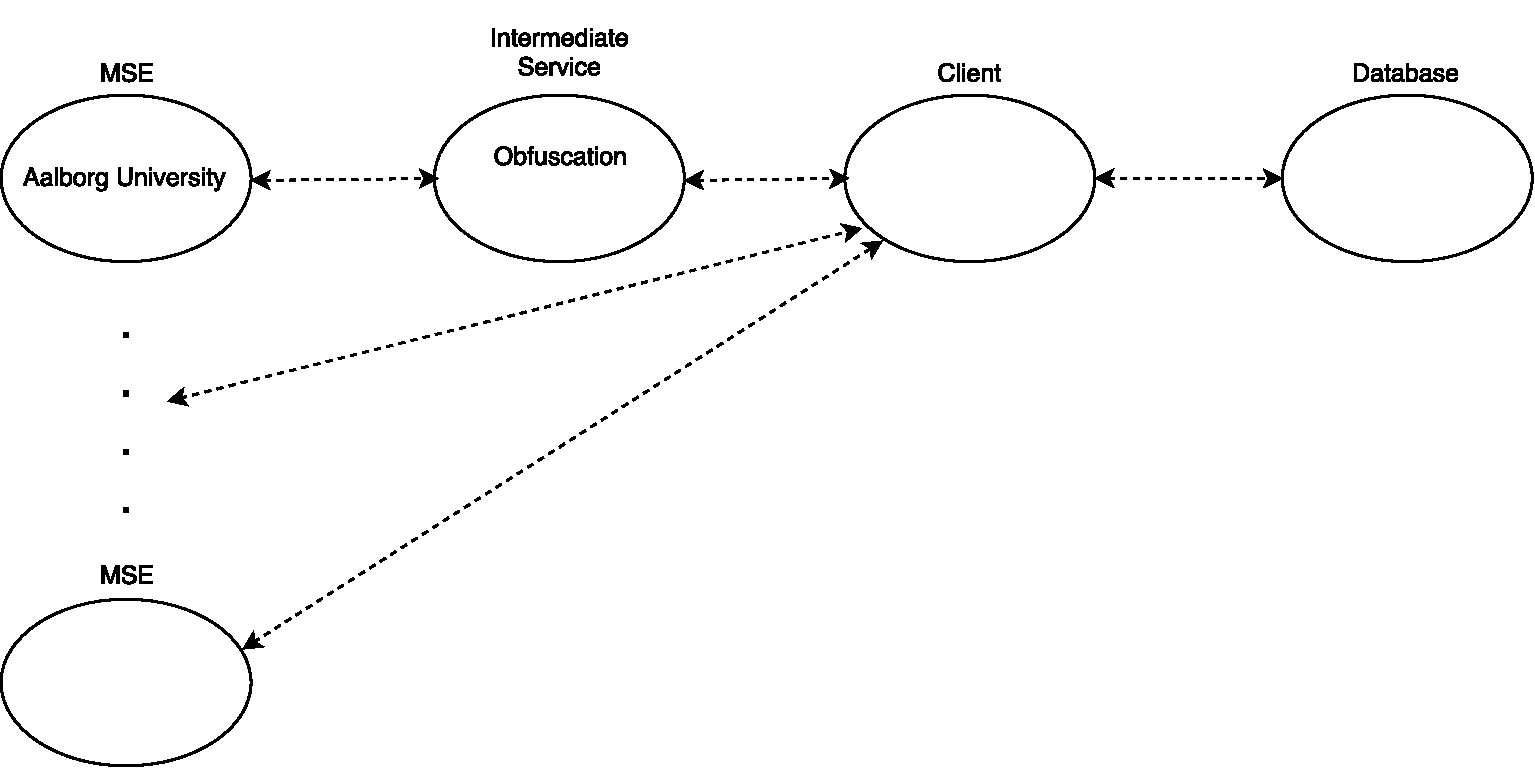
\includegraphics[scale=0.7]{graphics/ciscoNew.pdf}
		\caption{System data flow}
		\label{fig:system_flow}
	\end{center}
\end{figure}
The model shows how information is collected by the client from an arbitrary number of MSE services. After collecting the data, the client performs some operations and redirects the data to the database. The obfuscation will likewise also be performed by the client, as we wish to obfuscate person sensitive information from all MSE systems. It is possible for the database to communicate back to the client. For instance, a user may have agreed that we store their MAC address, which has to be communicated back to the client, such that the obfuscation algorithm takes this into account.

